\documentclass[11pt]{article}
\usepackage[utf8]{inputenc}
\usepackage[brazil]{babel}
\usepackage{graphicx}
\usepackage{tabularx}
\usepackage{cite}
\usepackage{listings}
\DeclareGraphicsExtensions{.pdf,.png,.jpg}
\setlength{\topmargin}{-.5in}
\setlength{\textheight}{9in}
\setlength{\oddsidemargin}{.125in}
\setlength{\textwidth}{6.25in}
\usepackage{xcolor,colortbl}
\definecolor{gray}{rgb}{0.85,0.85,0.85}
\definecolor{lightblue}{rgb}{0.75,0.75,0.75}

\begin{document}

  \begin{titlepage}
  
    \centering
    
\includegraphics[width=.5\textwidth]{logo.jpg}

    \vspace{\stretch{1}}
    \large{CURSO SUPERIOR DE TECNOLOGIA EM ANÁLISE E DESENVOLVIMENTO DE SISTEMAS, REDES DE COMPUTADORES E GESTÃO DE TECNOLOGIA DA INFORMAÇÃO}

    \vspace{\stretch{1}}

    \large{BRAUNER SOUZA DE MELLO\\DALMIR DA SILVA}

    \vspace{\stretch{1}}
    \large{\textbf{GRAFORM}}

    \vspace{\stretch{2}}
    \large{PORTO ALEGRE, \\DEZ de 2013}
    
  \end{titlepage}

  \newpage
  \thispagestyle{empty}
  \mbox{}
  
  \newpage
  
  \tableofcontents
  
  \newpage
  
  \listoffigures
  \listoftables

  \newpage
  
  \begin{abstract}
    Nos dias atuais, empresas que fornecem serviços de monitoramento de 
    indicadores e índices de satisfação de clientes, precisam de uma 
    solução de software que seja poderosa, e ao mesmo tempo, simples de 
    ser utilizada. Este é o caso da Stringhini Marketing. 
    Este trabalho propõe o desenvolvimento de um sistema de 
    gerenciamento de formulários eletrônicos, direcionado ao escopo de 
    negócio da Stringhini. O sistema, denominado Graform, tem, como 
    principal objetivo, o papel de substituir a forma como a Stringhini
    gerencia e entrega o seu serviço de questionários eletrônicos, 
    possibilitando que os mesmos deixem de ser criados e editados 
    diretamento na base de dados e passem a ter uma interface web, 
    simples e funcional. 
    Baseando-se em regras aplicadas a cada resposta de uma  questão do
    formulário, o sistema Graform permite controlar a ordem das 
    próximas questões, alterando o fluxo de respostas e customizando 
    o formulário como um todo. Possibilitando assim, coletar 
    informações mais relevantes do que um formulário convencional.
  \end{abstract}

  \newpage

  \section{Introdução}
  
    \subsection{A empresa}

      \paragraph{}
      
      A Stringhini Marketing é uma empresa de marketing com experiência 
      em gestão da operação comercial e do relacionamento com o cliente 
      através do monitoramento de indicadores chave e índices de 
      satisfação. A empresa dá muita importância à inteligência 
      competitiva e procura transformar informação em estratégia e 
      decisão em resultado, agregando valor ao negócio dos clientes.
      
    \subsection{Problema a ser resolvido}

      \paragraph{}

      Devido ao grande número de informações trabalhadas em uma pesquisa 
      de marketing, há uma grande dificuldade em não se ter uma 
      interface amigável de criação e gerenciamento de pesquisas.
      
      \paragraph{}
      
      O desenvolvimento dos formulários é diretamente no banco de 
      dados através de scripts, o que gerar um grande risco de 
      inconsistência pela possibilidade de erro humano, a dificuldade de 
      manutenção é muito alta, tornando a personalização de um 
      formulário quase impossível. No atual momento, a empresa não vê 
      condições de adquirir um software no mercado, por julgar que não 
      atende em relação aos custos e necessidades específicas de cada 
      projeto.
      
    \subsection{Objetivos do trabalho}

      \paragraph{}

      O objetivo do projeto é desenvolver uma ferramenta web para 
      criação e gerenciamento de pesquisas, com uma interface amigável e
      de uso fácil para os clientes. Com o desenvolvimento deste 
      software, a empresa permitirá autonomia aos clientes, pois os 
      mesmos terão condições de desenvolver suas pesquisas conforme sua 
      necessidade, bem como, possibilitará a que sua equipe tenha condições 
      de focar apenas na inteligência do negócio e não mais na operação.

  \newpage

  \section{Sistema}

    \subsection{Definição}
    
      \subsubsection{Funcionalidades}

      \paragraph{}
      
      O projeto em questão trata-se do desenvolvimento de um sistema 
      de  criação e gerenciamento de formulários eletrônicos online. A
      ferramenta consiste em uma página {\em web} onde os clientes da
      Stringhini poderão criar e gerenciar seus próprios formulários, 
      através de uma conta de usuário.
      
      \paragraph{}
      
      O sistema possui as seguintes características:

      \begin{enumerate}
        \item Provê uma interface web para manipulação dos formulários;
        \item Possibilita a criação de dois tipos distintos de formulários:
          \begin{enumerate}
            \item Condicional: A sequência das questões a serem 
            respondidas pode variar de acordo com as respostas;
            \item Contínuo: Possui sequência estática de questões;
          \end{enumerate}
        \item Usuários acessam os dados concorrentemente;
        \item Possui interface amigável, limpa e simples;
      \end{enumerate}
      
      \subsubsection{Modelagem}

        \paragraph{}
        
        Um formulário consiste em um conjunto de questões encadeadas de
        duas maneiras possíveis: contínua ou condicional.
        
        \paragraph{}
        
        Da forma contínua, as questões são respondidas pela ordem de 
        seus números. Por exemplo: a questão n$\textsuperscript{\underline{o}}$ 1 
        será a primeira a ser respondida, seguida pela questão n$\textsuperscript{\underline{o}}$ 2,
        n$\textsuperscript{\underline{o}}$ 3... e assim sucessivamente.
        
        \paragraph{}
        
        Quando o formulário for condicional, a sequência de questões 
        não segue, necessariamente, tal ordem. A sequência de questões
        é dinamicamente escolhida em função das respostas, isto é, 
        respostas diferentes podem determinar diferentes próximas 
        questões.
        
        \subparagraph{Grafo}
        
        \paragraph{}
        
        Para modelar o sistema, seguindo as características de condicionalidade
        citadas acima, os formulários são organizados internamente de uma maneira
        análoga a uma estrutura de dados chamada {\em grafo}. 
        
        \paragraph{}
        
        Um grafo é uma estrutura de dados $G(V,A)$, onde $V$ é um 
        conjunto não vazio de objetos 
        denominados vértices e $A$ é um conjunto de pares de $V$, 
        chamado arestas \cite{graphTenenbaum,graphMarcos}. Analogamente, 
        um formulário é uma estrutura $F(Q, R)$, onde $Q$ é um conjunto
        de questões e $R$ é um conjunto de pares de $Q$. $R$, sendo um conjunto de 
        pares ordenados, torna o grafo orientado.
        
        \paragraph{}
        
        Para uma dada questão $q \in Q$, a próxima questão $Q_k$ é determinada 
        pelas possíveis respostas $A$ de $q$ e uma regra $r$. Portanto, cada elemento
        de $R$ é definido como uma função que mapeia a questão atual, a 
        resposta e uma regra para uma próxiam questão: 
        
        \begin{eqnarray}
          R_n &=& f(q, A_n, r) : Q_k
        \end{eqnarray}
        
        Visualmente podemos perceber que, dependendo da resposta para 
        cada questão, pode-se percorrer diferentes regiões do formulário
        (grafo). A próxima figura representa tal formulário, onde $q_n$ são questões e $r_n$ são associações entre respostas 
        e regras para cada questão $q$.
        
        \begin{figure}[h!]
          \centering
          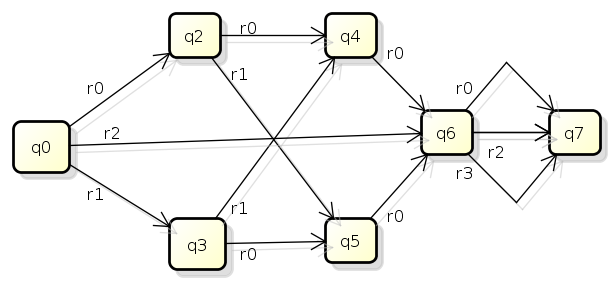
\includegraphics[width=.9\textwidth]{graph.png}
          \caption{Formulário visto como um grafo.}
        \end{figure}
          
        \paragraph{}
        
        Para controlar a primeira e última questão de um formulário, cada
        vértice contém 2 atributos: '{\em inicial}' e '{\em final}'. Pode haver
        apenas um vértice inicial. Entretanto, múltiplos vértices podem ser
        considerados terminais (finais), permitindo que o formulário seja 
        encerrado de forma controlada.
        
      \subsection{Tecnologias escolhidas}
        
        \paragraph{}
        
        Devido ao apoio da instituição, onde esse trabalho foi realizado,
        à projetos e iniciativas {\em open source}, decidiu-se utilizar,
        em todas as partes desse trabalho, ferramentas livres e/ou de código fonte aberto.
        Desde o sistema operaconal onde ele foi desenvolvido até
        o programa utilizado para escrever esse documento.
        
        \subsubsection{Sistema Operacional}

          \paragraph{}
          
          O Sistema Operacional (SO) utilizado é o Linux. Mais 
          precisamente a distribuição Ubuntu \cite{website:ubuntu}, de código aberto, 
          construído a partir do núcleo Linux, baseado no Debian.
          
        \subsubsection{Versionamento}

          \paragraph{}
          
          O sistema desenvolvido utiliza o Git. Git é um sistema de 
          controle de versão distribuído e um sistema de gerenciamento 
          de código fonte, com ênfase em velocidade. O Git foi inicialmente 
          projetado e desenvolvido por Linus Torvalds para o desenvolvimento 
          do kernel Linux, mas foi adotado por muitos outros projetos \cite{website:git}.
          
        \subsubsection{Produção de textos científicos}

          \paragraph{}
          
          Fugindo do senso comum, utilizou-se o {\LaTeX} para escrever esse 
          documento. {\LaTeX} é utilizado amplamente 
          para a produção de textos matemáticos e científicos devido à 
          sua alta qualidade tipográfica \cite{website:latex}.
          
        \subsubsection{{\em Framework} de desenvolvimento}

          \paragraph{}
          
          Levando em consideração as características do sistema e a ideia de 
          criar a aplicação utilizando a arquitetura MVC (Model-View-Controler), 
          decidiu-se implementar o sistema Graform usando o {\em framework }
          livre Ruby on Rails, projeto  de código 
          aberto escrito na linguagem Ruby. Ruby on Rails foi uma 
          extração de David Heinemeier Hansson de um projeto seu, o 
          gerenciador de projetos Basecamp \cite{website:rails,urubatan,thomas}. 
          Foi lançado a público pela primeira vez em julho de 2004.
          
        \subsubsection{Linguagem de programação}

          \paragraph{}
          
          Por termos optado pelo {\em framework} Ruby on Rails, a linguagem 
          escolhida foi, obviamente, o Ruby. Uma 
          linguagem dinâmica, open source com foco na simplicidade e na 
          produtividade \cite{website:ruby}.
          
        \subsubsection{Biblioteca {\em javascript}}

          \paragraph{}
          
          Como biblioteca {\em javascript}, o jQuery \cite{website:jquery} foi 
          utilizado, devido a sua simplicidade e capacidade de funcionar em diferentes
          navegadores. 
          
        \subsubsection{Servidor web}

          \paragraph{}
          
          O servidor web escolhido foi o Nginx, em detrimento do Apache, devido ao fato de
          o Nginx ser um servidor web rápido, leve, e com inúmeras 
          possibilidades de configuração para melhor performance.
          Técnicamente, o Nginx consome menos memória que o Apache, 
          pois lida com requisições Web através do conceito de 
          {\em event-based web server}, já o Apache é baseado no 
          conceito {\em process-based server} \cite{website:nginx}. 
          
        \subsubsection{Servidor de banco de dados}

          \paragraph{}
          
          O servidor de banco de dados utilizado é o MySQL. 
          O MySQL é um sistema de gerenciamento de banco de dados (SGBD), 
          que utiliza a linguagem SQL (Linguagem de Consulta Estruturada, 
          do inglês {\em Structured Query Language}) como interface. 
          É atualmente um dos bancos de dados mais populares, 
          com mais de 10 milhões de instalações pelo mundo \cite{website:mysql}.
  
  \clearpage
  
      \subsection{Análise das soluções existentes}

      \paragraph{}

      Para o presente trabalho, pesquisamos os principais fornecedores de 
      funcionalidades similares no mercado. Três fornecedores foram 
      identificados como os mais áptos a fornecer os serviços desejados
      pela Stringhini. São eles:

      \begin{enumerate}
        \item Surveymonkey \cite{website:surveymonkey};
        \item Eval \& Go\cite{website:evalgo};
        \item Google Forms\cite{website:googleforms}.
      \end{enumerate}

      \paragraph{}
      
      Dentre os fornecedores acima citados, pesquisamos as 
      funcionalidades mais relevantes providas pelos mesmo. Como segue:

      \begin{enumerate}
        \item Cadastro de opções de respostas;
        \item Alterar questões de acordo com o tipo de respostas;
        \item Preço acessível;
        \item Reaproveitar formulários.
      \end{enumerate}

      \paragraph{}
      
      No quadro abaixo, consta o comparativo de funcionalidades entre os 
      fornecedores de serviços de formulários online escolhidos, também
      os serviços que o projeto Graform propõem desenvolver.

      \paragraph{}

      \begin{table}[h]
        \begin{center}
          \begin{tabular}{ | p{5cm} | c | c | c | c | }
            \hline
                                                                                & Surveymonkey\cellcolor{gray}  & Eval \& Go\cellcolor{gray} & Google\cellcolor{gray} & \em Graform\cellcolor{gray} \\
            \hline
            Cadastro de opções de respostas\cellcolor{gray}                     & X             & X           & X       & \em X \\
            \hline
            Alterar questões de acordo com o tipo de respostas\cellcolor{gray} & X             & X           &         & \em X \\
            \hline
            Preço acessível\cellcolor{gray}                                     &               &             & X       & \em X \\
            \hline
            Reaproveitar formulários\cellcolor{gray}                          &               & X           &         & \em X \\
            \hline
          \end{tabular}
          \caption{Comparativo de funcionalidades.}
        \end{center}
      \end{table}
      
  \newpage

  \section{Especificação dos requisitos}
    
    \subsection{Requisitos Funcionais}

    \paragraph{}
    As especificações a seguir mostram, detalhadamente, cada requisito funcional.
    
      \subsubsection{Cadastrar usuário.}
      
        \begin{table}[h]
          \begin{center}
              \begin{tabular}{ | p{5cm} | p{10cm} | }
                \hline
                Código\cellcolor{gray} & RF. 001\cellcolor{gray} \\
                \hline
                Título & Cadastrar usuário. \\
                \hline
                Descrição & Cadastrar um usuário no sistema. \\
                \hline
                Pré-condições & Nenhuma. \\
                \hline
                Pós-condições & Ir para tela de login. \\
                \hline
                Cenários &   \\
                \hline
                1.  Cenário Principal & Um usuário ainda não cadastrado acessa a área de Sign up \\
                \hline
              \end{tabular}
            \caption{RF. 001 - Cadastrar usuário.}
          \end{center}
        \end{table}

      \subsubsection{Autenticar usuário no sistema.}

        \begin{table}[h]
          \begin{center}
            \begin{tabular}{ | p{5cm} | p{10cm} | }
              \hline
              Código\cellcolor{gray} & RF. 002\cellcolor{gray} \\
              \hline
              Título & Autenticar usuário no sistema. \\
              \hline
              Descrição & Autenticar um usuário cadastrado no sistema. \\
              \hline
              Pré-condições & Usuário estar previamente cadastrado. \\
              \hline
              Pós-condições & Listar formulários do usuário. \\
              \hline
              Cenários &   \\
              \hline
              1.  Cenário Principal & Usuário acessa a área de Login. \\
              \hline
              2.  Cenário Alternativo & Usuário tenta acessar qualquer área restrita do site. \\
              \hline
            \end{tabular}
            \caption{RF. 002 - Autenticar usuário no sistema.}
          \end{center}
        \end{table}

    \clearpage

      \subsubsection{Cadastrar formulário.}

        \begin{table}[h]
          \begin{center}
            \begin{tabular}{ | p{5cm} | p{10cm} | }
              \hline
              Código\cellcolor{gray} & RF. 003\cellcolor{gray} \\
              \hline
              Título & Cadastrar formulário. \\
              \hline
              Descrição & Cadastrar um formulário no sistema associado a um usuário. \\
              \hline
              Pré-condições & Usuário estar logado no sistema. \\
              \hline
              Pós-condições & Lista de formulários cadastrados no sistema associados ao usuário logado. \\
              \hline
              Cenários &   \\
              \hline
              1.  Cenário Principal & Usuário realiza a inserção de um novo formulário no sistema, associando-o automaticamente a si. \\
              \hline
            \end{tabular}
            \caption{RF. 003 - Cadastrar formulário.}
          \end{center}
        \end{table}
    
      \subsubsection{Editar formulário.}

        \begin{table}[h]
          \begin{center}
            \begin{tabular}{ | p{5cm} | p{10cm} | }
              \hline
              Código\cellcolor{gray} & RF. 004\cellcolor{gray} \\
              \hline
              Título & Editar formulário. \\
              \hline
              Descrição & Editar um formulário existente. Incluindo a adição de novas questões e opções. \\
              \hline
              Pré-condições & Usuário estar logado no sistema, existir um formulário. \\
              \hline
              Pós-condições & Cuntinuar na tela de edição. \\
              \hline
              Cenários & \\
              \hline
              1.  Cenário Principal & Usuário solicita tela de edição de formulário. Nessa tela, é possível adicionar, remover, e editar questões. \\
              \hline
            \end{tabular}
            \caption{RF. 004 - Editar formulário.}
          \end{center}
        \end{table}

    \clearpage
  
      \subsubsection{Cadastrar questão.}

        \begin{table}[h]
          \begin{center}
            \begin{tabular}{ | p{5cm} | p{10cm} | }
              \hline
              Código\cellcolor{gray} & RF. 005\cellcolor{gray} \\
              \hline
              Título & Cadastrar questão. \\
              \hline
              Descrição & Cadastrar uma nova questão no sistema associada a um formulário. \\
              \hline
              Pré-condições & Existir um formulário. Estar na tela de edição desse formulário. \\
              \hline
              Pós-condições & N/A \\
              \hline
              Cenários &   \\
              \hline
              1.  Cenário Principal & Usuário está na tela de edição de um formulário, solicita a inclusão de uma nova questão ao formulário. \\
              \hline
            \end{tabular}
            \caption{RF. 005 - Cadastrar questão.}
          \end{center}
        \end{table}

      \subsubsection{Cadastrar opção.}

        \begin{table}[h]
          \begin{center}
            \begin{tabular}{ | p{5cm} | p{10cm} | }
              \hline
              Código\cellcolor{gray} & RF. 006\cellcolor{gray} \\
              \hline
              Título & Cadastrar opção. \\
              \hline
              Descrição & Um usuário edita um formulário. Para as questões do tipo Multipla Escolha e Única Escolha, o usuário solicita a inclusão de uma nova opção para uma dada questão. \\
              \hline
              Pré-condições & Existir uma questão cadastrada no sistema. \\
              \hline
              Cenários &   \\
              \hline
              1.  Cenário Principal & Usuário insere uma nova opção. \\
              \hline
            \end{tabular}
            \caption{RF. 006 - Cadastrar opção.}
          \end{center}
        \end{table}

    \clearpage

      \subsubsection{Responder um formulário.}

        \begin{table}[h]
          \begin{center}
            \begin{tabular}{ | p{5cm} | p{10cm} | }
              \hline
              Código\cellcolor{gray} & RF. 007\cellcolor{gray} \\
              \hline
              Título & Responder um formulário. \\
              \hline
              Descrição & Responder um fomulário. Pode ser realizado por um usuário anônimo ou um usuário cadastrado no sistema. \\
              \hline
              Pré-condições & Existir um formulário no sistema. \\
              \hline
              Pós-condições & Tela de agradecimento. \\
              \hline
              Cenários &   \\
              \hline
              1.  Cenário Principal & Acesso ao link de resposta de um fomrulário. \\
              \hline
            \end{tabular}
            \caption{RF. 007 - Responder um formulário.}
          \end{center}
        \end{table}
    
      \subsubsection{Visualizar as respostas de um formulário.}

        \begin{table}[h]
          \begin{center}
            \begin{tabular}{ | p{5cm} | p{10cm} | }
              \hline
              Código\cellcolor{gray} & RF. 008\cellcolor{gray} \\
              \hline
              Título & Visualizar as respostas de um formulário. \\
              \hline
              Descrição & O usuário dono do formulário poderá acessar a pagina de relatório r visualizar todas as respostas de uma dado formulário. \\
              \hline
              Pré-condições & Existir um formulário cadastrado no sistema. \\
              \hline
              Pós-condições & N/A \\
              \hline
              Cenários &   \\
              \hline
              1.  Cenário Principal & Usuário acessa a área de relatorios, escolhe um formulário para ser visualizado. \\
              \hline
              2.  Cenário Alternativo & Usuário com um formulário cadastrado no sistema, acessa esse formulário e solicita a visualização do relatório desse formulário. \\
              \hline
            \end{tabular}
            \caption{RF. 008 - Visualizar as respostas de um formulário.}
          \end{center}
        \end{table}

    \clearpage

    \subsection{Requisitos não Funcionais}
    
      \paragraph{}
      As especificações a seguir mostram os requisitos não funcionais do sistema.

      \subsubsection{Utilizar a nuvem da Amazon.}

        \begin{table}[h]
          \begin{center}
            \begin{tabular}{ | p{5cm} | p{10cm} | }
              \hline
              Código\cellcolor{gray} & RNF. 001\cellcolor{gray} \\
              \hline
              Título & Utilizar a nuvem da Amazon. \\
              \hline
              Descrição & Toda a aplicação deverá rodar usando a infraestrutura de nuvem da Amazon. \\
              \hline
            \end{tabular}
            \caption{RNF. 001 - Utilizar a nuvem da Amazon.}
          \end{center}
        \end{table}

      \subsubsection{Utilizar máquina como servidor de aplicação.}

        \begin{table}[h]
          \begin{center}
            \begin{tabular}{ | p{5cm} | p{10cm} | }
              \hline
              Código\cellcolor{gray} & RNF. 002\cellcolor{gray} \\
              \hline
              Título & Utilizar máquina como servidor de aplicação. \\
              \hline
              Descrição & Será utilizado uma instância do tipo micro na nuvem da Amazon como servidor de aplicação. \\
              \hline
            \end{tabular}
            \caption{RNF. 002 - Utilizar máquina como servidor de aplicação.}
          \end{center}
        \end{table}

      \subsubsection{Utilizar máquina como servidor de banco de dados.}

        \begin{table}[h]
          \begin{center}
            \begin{tabular}{ | p{5cm} | p{10cm} | }
              \hline
              Código\cellcolor{gray} & RNF. 003\cellcolor{gray} \\
              \hline
              Título & Utilizar máquina como servidor de banco de dados. \\
              \hline
              Descrição & Será utilizado uma instância do tipo micro na nuvem da Amazon como servidor de banco de dados. \\
              \hline
            \end{tabular}
            \caption{RNF. 003 - Utilizar máquina como servidor de banco de dados.}
          \end{center}
        \end{table}

    \clearpage

      \subsubsection{Utilizar servidor de banco de dados MySQL.}

        \begin{table}[h]
          \begin{center}
            \begin{tabular}{ | p{5cm} | p{10cm} | }
              \hline
              Código\cellcolor{gray} & RNF. 004\cellcolor{gray} \\
              \hline
              Título & Utilizar servidor de banco de dados MySQL. \\
              \hline
              Descrição & Será utilizado o MySQL como servidor de banco de dados. \\
              \hline
            \end{tabular}
            \caption{RNF. 004 - Utilizar servidor de banco de dados MySQL.}
          \end{center}
        \end{table}

      \subsubsection{Utilizar o nginx como servidor web.}

        \begin{table}[h]
          \begin{center}
            \begin{tabular}{ | p{5cm} | p{10cm} | }
              \hline
              Código\cellcolor{gray} & RNF. 005\cellcolor{gray} \\
              \hline
              Título & Utilizar o nginx como servidor web. \\
              \hline
              Descrição & Será utilizado o nginx como servidor web. \\
              \hline
            \end{tabular}
            \caption{RNF. 005 - Utilizar o nginx como servidor web.}
          \end{center}
        \end{table}

      \subsubsection{Utilizar a linguagem Ruby.}

        \begin{table}[h]
          \begin{center}
            \begin{tabular}{ | p{5cm} | p{10cm} | }
              \hline
              Código\cellcolor{gray} & RNF. 006\cellcolor{gray} \\
              \hline
              Título & Utilizar a linguagem Ruby. \\
              \hline
              Descrição & Será utilizado a linguagem Ruby para o desenvolvimento da aplicação. \\
              \hline
            \end{tabular}
            \caption{RNF. 006 - Utilizar a linguagem Ruby.}
          \end{center}
        \end{table}

    \clearpage
        
      \subsubsection{Utilizar o framework Ruby on Rails.}

        \begin{table}[h]
          \begin{center}
            \begin{tabular}{ | p{5cm} | p{10cm} | }
              \hline
              Código\cellcolor{gray} & RNF. 007\cellcolor{gray} \\
              \hline
              Título & Utilizar o framework Ruby on Rails. \\
              \hline
              Descrição & Será utilizado o framework Ruby on Rails para o desenvolvimento da aplicação. \\
              \hline
            \end{tabular}
            \caption{RNF. 007 - Utilizar o framework Ruby on Rails.}
          \end{center}
        \end{table}

    \clearpage

    \subsection{Casos de uso}
      
      \subsubsection{Cadastrar usuário.}

        \begin{figure}[h!]
          \centering
          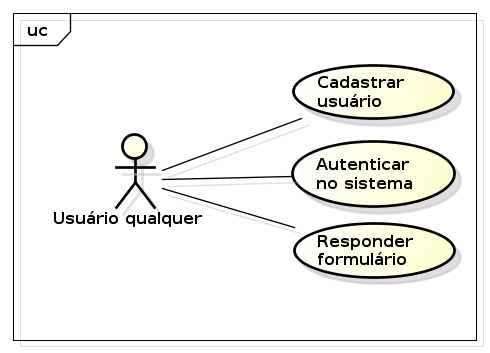
\includegraphics[width=.5\textwidth]{auth_create_user.png}
          \caption{Cadastrar usuário}
        \end{figure}

        \begin{table}[h]
          \begin{center}
            \begin{tabular}{ | p{7cm} | p{8cm} | }
              \hline
              Código: \cellcolor{gray} & UC01. \\
              \hline
              Nome do UC: \cellcolor{gray} & Cadastrar usuário. \\
              \hline
              Objetivo: \cellcolor{gray} & Registrar um novo usuário no sistema. \\
              \hline
              Ativação: \cellcolor{gray} & Página principal / \em Sign up \\
              \hline
              \hline
              Cenário 1 - Cadastrar um usuário: &  \\
              \hline
              Ação\cellcolor{gray} & Reação\cellcolor{gray} \\
              \hline
              Um usuário ainda não cadastrado clica no \em link Sign up & O sistema exibe um formulário para o usuário entrar com as informações. \\
              \hline
              O usuário entra com os dados. E clica no botão ‘Registrar’. & O sistema valida as informações. Insere o novo usuário e redireciona para a página de login. Em caso de falha, exibe mensagem de erro na tela. \\
              \hline
              \hline
              Cenário 2 - Visualizar usuário: &  \\
              \hline
              Ação\cellcolor{gray} & Reação\cellcolor{gray} \\
              \hline
              O usuário já cadastrado e logado no sistema, clicar no link 'Minha conta'. & O sistema exibe as informações do usuário. \\
              \hline
            \end{tabular}
            \caption{UC01 - Cadastrar usuário.}
          \end{center}
        \end{table}

    \clearpage

      \subsubsection{Autenticar usuário no sistema.}

        \begin{figure}[h!]
          \centering
          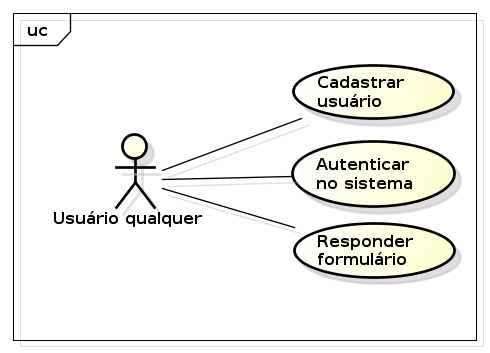
\includegraphics[width=.5\textwidth]{auth_create_user.png}
          \caption{Autenticar usuário no sistema}
        \end{figure}

        \begin{table}[h]
          \begin{center}
            \begin{tabular}{ | p{7cm} | p{8cm} | }
              \hline
              Código: \cellcolor{gray} & UC02. \\
              \hline
              Nome do UC: \cellcolor{gray} & Autenticar usuário no sistema. \\
              \hline
              Objetivo: \cellcolor{gray} & Autenticar um usuário existente no sistema. \\
              \hline
              Ativação: \cellcolor{gray} & Página principal / \em Login \\
              \hline
              \hline
              Cenário 1 - Autenticar um usuário: &  \\
              \hline
              Ação\cellcolor{gray} & Reação\cellcolor{gray} \\
              \hline
              Um usuário clica no \em link Login & O sistema exibe um formulário para o usuário entrar com as informações. \\
              \hline
              O usuário entra com os dados. E clica no botão 'Login'. & O sistema valida as informações. Autentica o usuário e redireciona para a página de lista de formulários. Em caso de falha, exibe mensagem de erro na tela. \\
              \hline
            \end{tabular}
            \caption{UC02 - Autenticar usuário no sistema.}
          \end{center}
        \end{table}

    \clearpage

      \subsubsection{Cadastrar formulário.}

        \begin{figure}[h!]
          \centering
          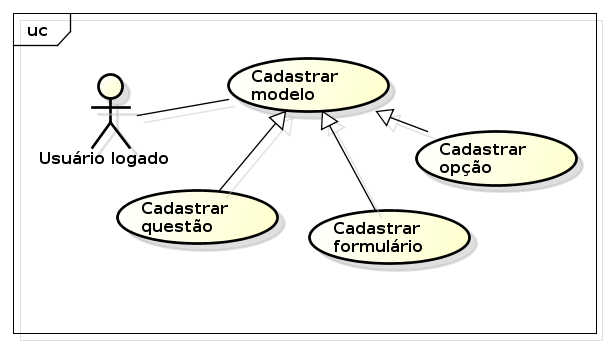
\includegraphics[width=.5\textwidth]{cadastrar.png}
          \caption{Cadastrar formulário}
        \end{figure}

        \begin{table}[h]
          \begin{center}
            \begin{tabular}{ | p{7cm} | p{8cm} | }
              \hline
              Código: \cellcolor{gray} & UC03. \\
              \hline
              Nome do UC: \cellcolor{gray} & Cadastrar formulário. \\
              \hline
              Objetivo: \cellcolor{gray} & Cadastrar um novo formulário no sitema. \\
              \hline
              Ativação: \cellcolor{gray} & Página principal / Meus formulários / Novo formulário \\
              \hline
              \hline
              Cenário 1 - Cadastrar um formulário: &  \\
              \hline
              Ação\cellcolor{gray} & Reação\cellcolor{gray} \\
              \hline
              Um usuário clica no botão 'Novo formulário' & O sistema exibe um formulário para o usuário entrar com as informações do novo formulário. \\
              \hline
              O usuário entra com os dados. E clica no botão 'Salvar'. & O sistema valida as informações, salva o formulário e redireciona para a página de edição do formulário. Em caso de falha, exibe mensagem de erro na tela. \\
              \hline
            \end{tabular}
            \caption{UC03 - Cadastrar formulário.}
          \end{center}
        \end{table}

    \clearpage
      
      \subsubsection{Editar formulário.}

        \begin{figure}[h!]
          \centering
          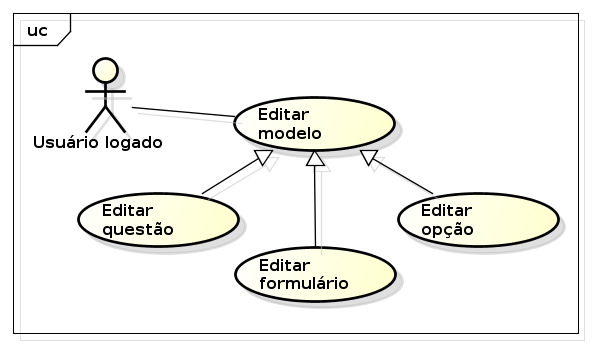
\includegraphics[width=.5\textwidth]{editar.png}
          \caption{Editar formulário}
        \end{figure}

        \begin{table}[h]
          \begin{center}
            \begin{tabular}{ | p{7cm} | p{8cm} | }
              \hline
              Código: \cellcolor{gray} & UC04. \\
              \hline
              Nome do UC: \cellcolor{gray} & Editar formulário. \\
              \hline
              Objetivo: \cellcolor{gray} & Editar um formulário existente no sitema. \\
              \hline
              Ativação: \cellcolor{gray} & Página principal / Formulário / Editor \\
              \hline
              \hline
              Cenário 1 - Editar um formulário: &  \\
              \hline
              Ação\cellcolor{gray} & Reação\cellcolor{gray} \\
              \hline
              Um usuário clica no botão 'Editor' & O sistema exibe as informações do formulário e uma lista de tipos de questão a ser adicionadas ao formulário. \\
              \hline
              O usuário clica no botão 'Adicionar', de um tipo específico de questão. & O sistema insere na tela um formulário para o usuário entrar com os dados da questão. Esse formulário deverá ser adicionado no final do formulário. \\
              \hline
              O usuário entra com o nome da questão e clica em salvar. & O sistema salva a questão, e exibe o feedback para o usuário. Sem recarregar a página. \\
              \hline
              O usuário clica no botão 'Adicionar' uma opção. & O sistema insere na tela uma opção para o usuário entrar com os dados. \\
              \hline
              O usuário entra com o valor da opção e clica em salvar. & O sistema salva a opção, e exibe o feedback para o usuário. Sem recarregar a página. \\
              \hline
            \end{tabular}
            \caption{UC04 - Editar formulário.}
          \end{center}
        \end{table}

    \clearpage
      
      \subsubsection{Responder um formulário.}

        \begin{figure}[h!]
          \centering
          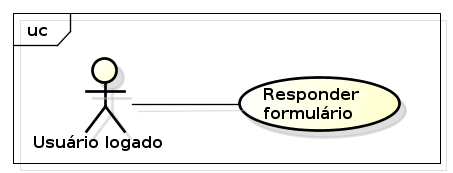
\includegraphics[width=.5\textwidth]{responder.png}
          \caption{Responder um formulário}
        \end{figure}

        \begin{table}[h]
          \begin{center}
            \begin{tabular}{ | p{7cm} | p{8cm} | }
              \hline
              Código: \cellcolor{gray} & UC05. \\
              \hline
              Nome do UC: \cellcolor{gray} & Responder um formulário. \\
              \hline
              Objetivo: \cellcolor{gray} & Coletar as respostas para um dado formulário. \\
              \hline
              Ativação: \cellcolor{gray} & Página principal / Formulário / Nova resposta \\
              \hline
              \hline
              Cenário 1 - Responder a um formulário do tipo contínuo: &  \\
              \hline
              Ação\cellcolor{gray} & Reação\cellcolor{gray} \\
              \hline
              Um usuário clica no {\em link} para responder o formulário & O sitema exibe as informações do formulário e todas as questões desse formulário. \\
              \hline
              O usuário responde cada pergunta e clica no botão 'Salvar' no final da lista de questões. & O sistema valida as respostas, salva todas e mostra a tela de agradecimento. Exibe mensagem de erro caso a validação não passe ou algum erro aconteça. \\
              \hline
              \hline              
              Cenário 2 - Responder a um formulário do tipo condicional: &  \\
              \hline
              Ação\cellcolor{gray} & Reação\cellcolor{gray} \\
              \hline
              Um usuário clica no {\em link} para responder o formulário & O sitema exibe as informações do formulário e a primeira questão do formulário. \\
              \hline
              O usuário responde a questão e clica em 'Próxima questão'. & O sistema valida a resposta e exibe a próxima questão. Exibe mensagem de erro caso ocorra. \\
              \hline
            \end{tabular}
            \caption{UC05 - Responder um formulário.}
          \end{center}
        \end{table}

    \clearpage
      
      \subsubsection{Visualizar relatório.}

        \begin{figure}[h!]
          \centering
          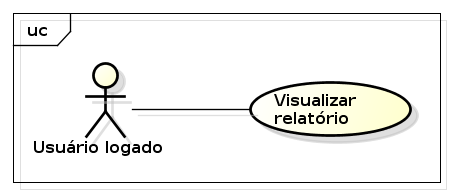
\includegraphics[width=.5\textwidth]{visualizar.png}
          \caption{Visualizar relatório}
        \end{figure}

        \begin{table}[h]
          \begin{center}
            \begin{tabular}{ | p{7cm} | p{8cm} | }
              \hline
              Código: \cellcolor{gray} & UC06. \\
              \hline
              Nome do UC: \cellcolor{gray} & Visualizar relatório. \\
              \hline
              Objetivo: \cellcolor{gray} & Relatar todas as respostas para uma dado formulário. \\
              \hline
              Ativação: \cellcolor{gray} & Página principal / Formulário / Relatório \\
              \hline
              \hline
              Cenário 1 - Responder a um formulário do tipo contínuo: &  \\
              \hline
              Ação\cellcolor{gray} & Reação\cellcolor{gray} \\
              \hline
              Um usuário logado, com um formulário, clica no {\em link} 'Relatório'. & O sitema exibe as respostas do formulário. \\
              \hline
            \end{tabular}
            \caption{UC06 - Visualizar relatório.}
          \end{center}
        \end{table}
        
  \clearpage
      
  \section{Diagramas}
  
    \subsection{Diagrama de classes}
    
      \paragraph{}
      O seguinte diagrama mostra as classes do sistema e suas cardinalidades.
    
      \begin{figure}[h!]
        \centering
        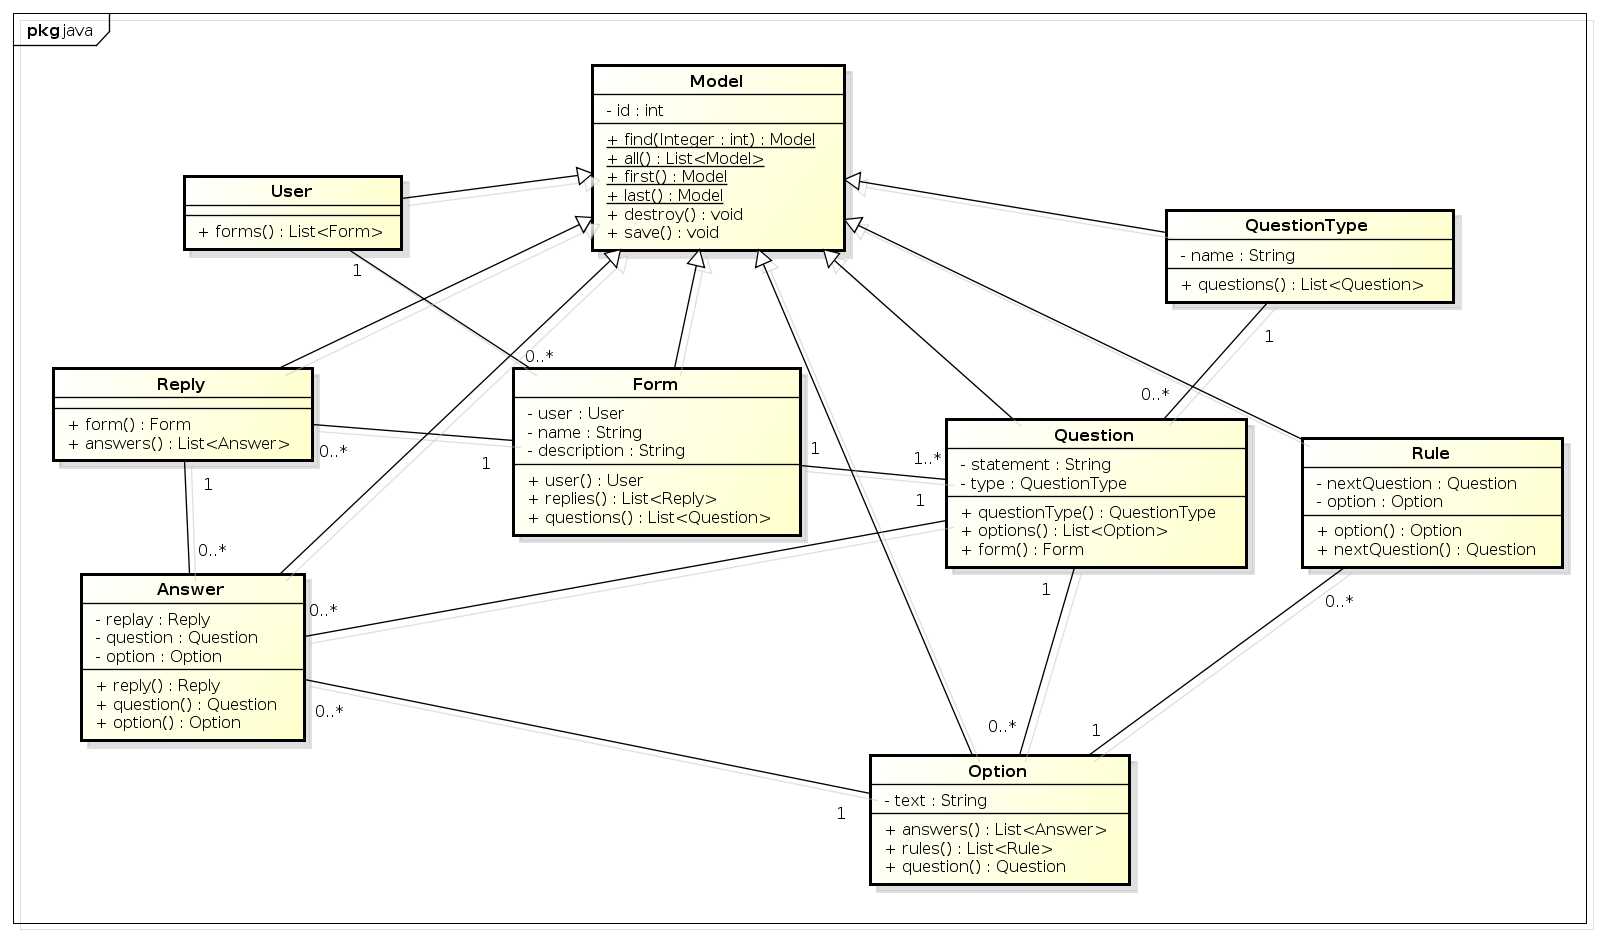
\includegraphics[width=1.0\textwidth]{class_diagram.png}
        \caption{Diagrama de classes}
      \end{figure}
        
  \clearpage
  
    \subsection{Diagramas de sequência}
    
      \subsubsection{Diagrama de sequência da interface REST da aplicação.}
    
      \paragraph{}
      O próximo diagrama descreve a sequência de comunicação entre o cliente - navegador, e o 
      serviço REST da aplicação.

        \begin{figure}[h!]
          \centering
          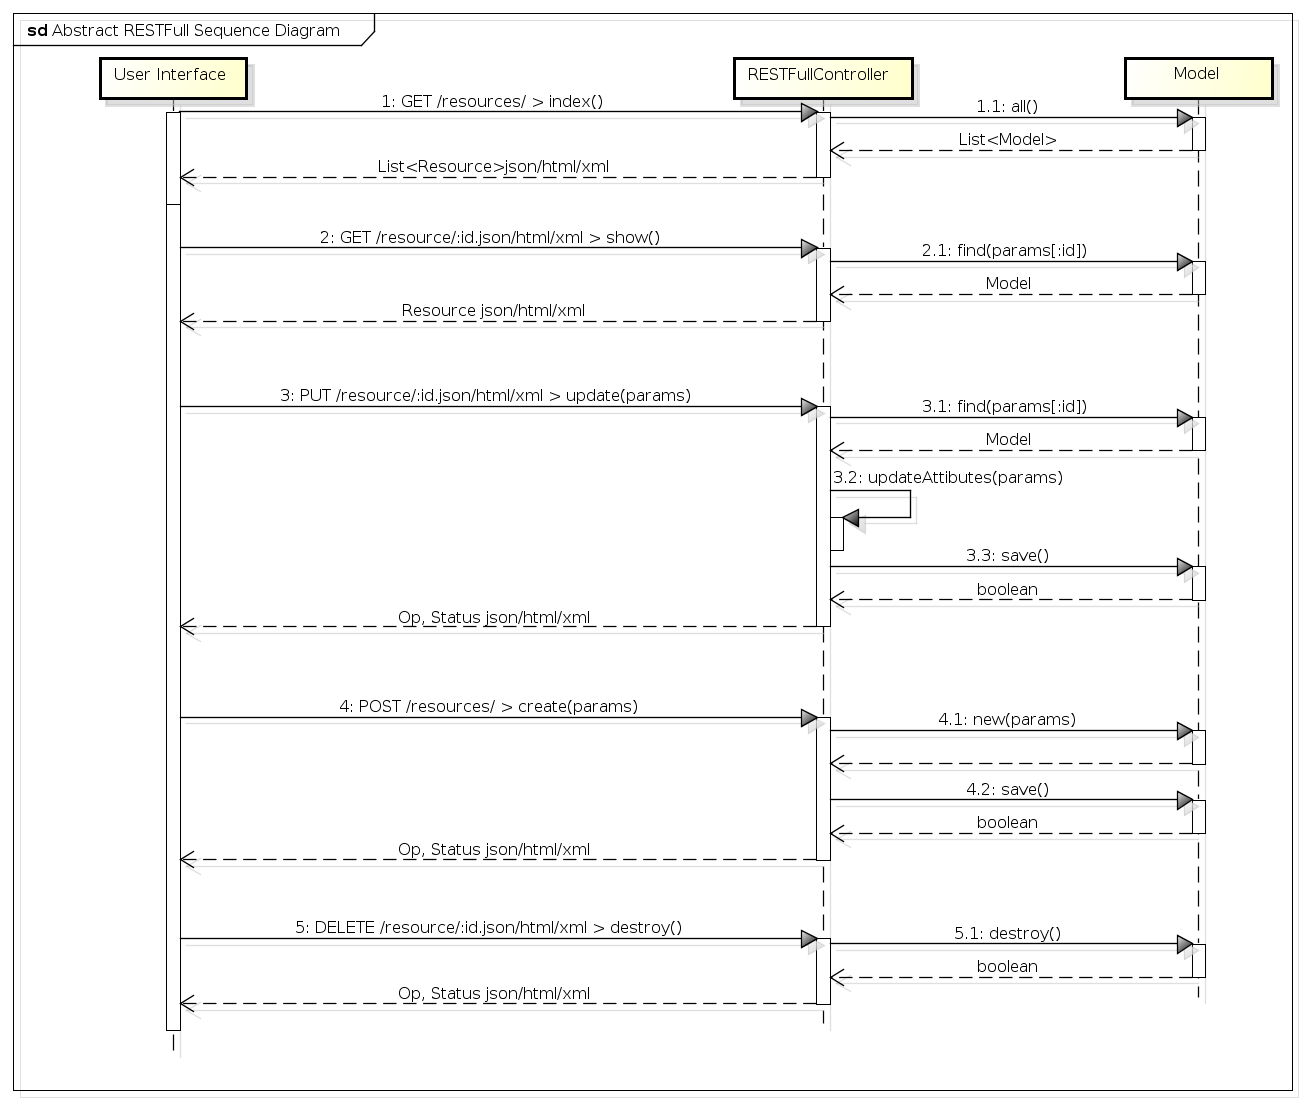
\includegraphics[width=1.0\textwidth]{sequence_diagram_main.png}
          \caption{Diagrama de sequência REST}
        \end{figure}
        
  \clearpage
    
      \subsubsection{Diagrama de sequência da edição de formulário da aplicação.}
    
      \paragraph{}
      O próximo diagrama descreve a sequência de comunicação para edição do 
      formulário.

        \begin{figure}[h!]
          \centering
          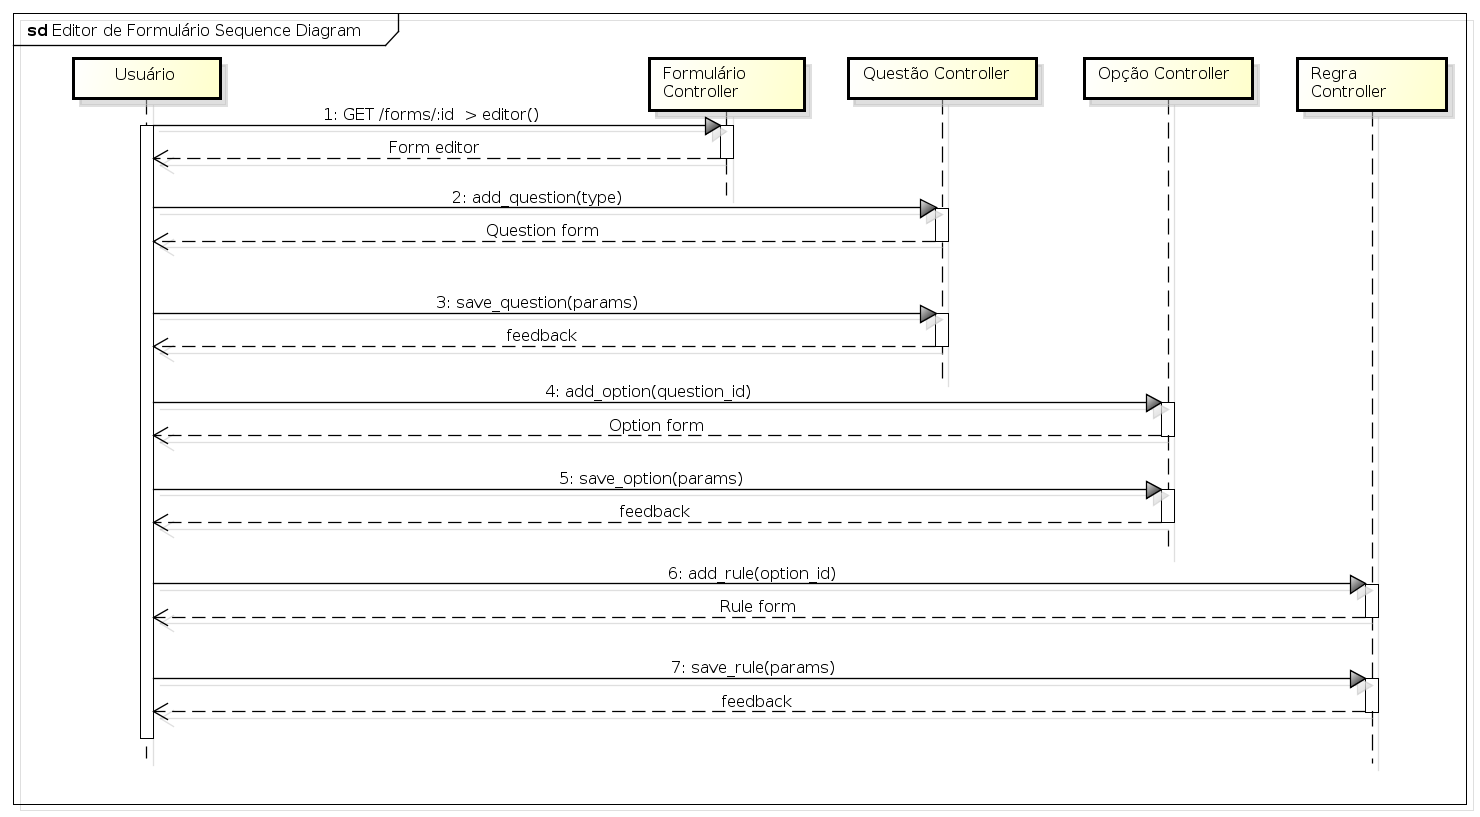
\includegraphics[width=1.0\textwidth]{sequence_diagram_editor.png}
          \caption{Diagrama de sequência da edição de formuário.}
        \end{figure}
        
  \clearpage
  
    \subsection{Diagrama entidade relacionamento}
    
    \paragraph{}
    O próximo modelo diagramático descreve, de forma abstrata, o modelo de dados do sistema.

      \begin{figure}[h!]
        \centering
        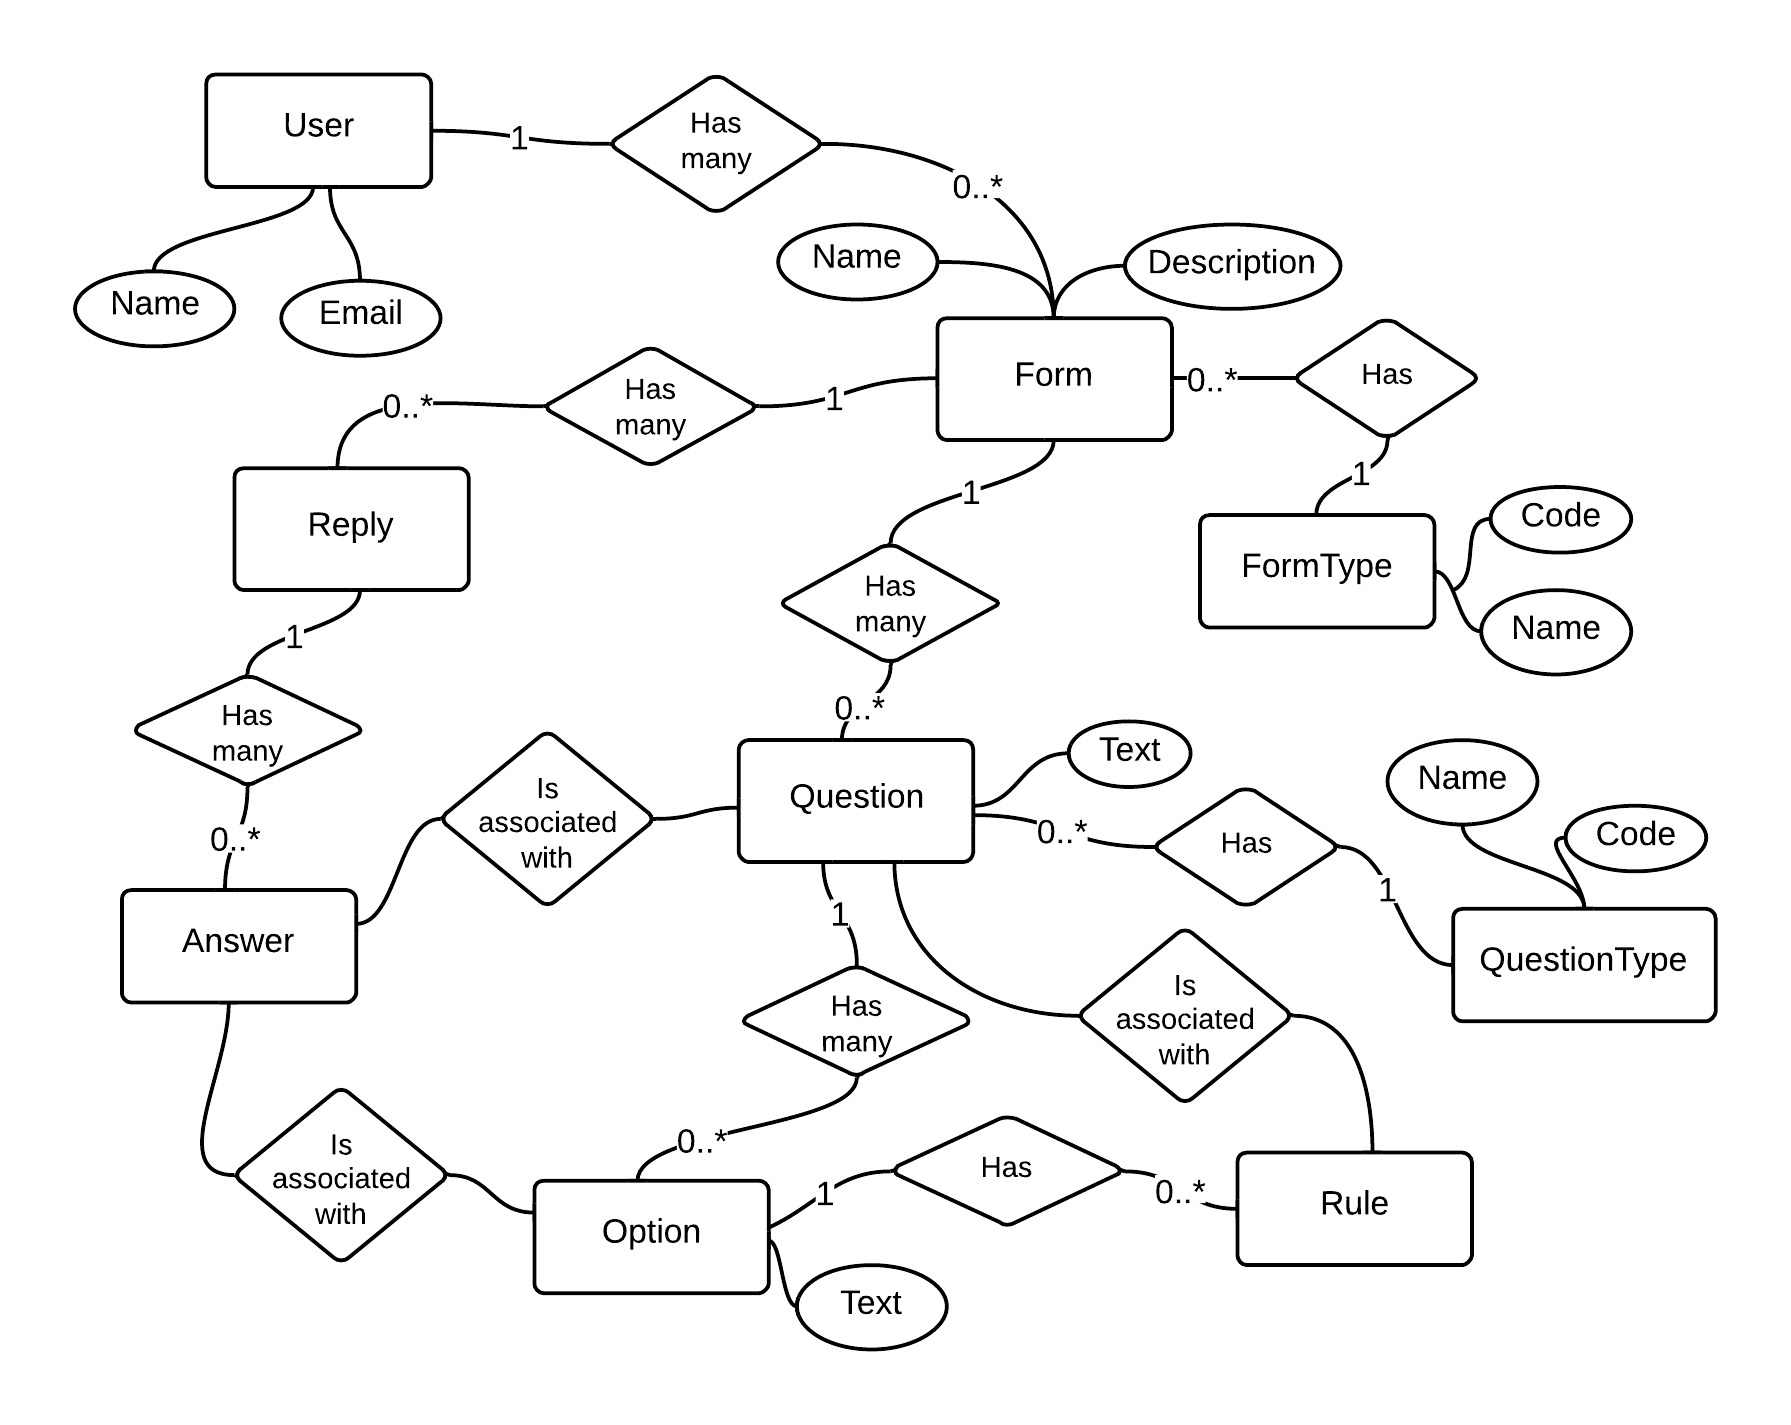
\includegraphics[width=1.0\textwidth]{er.png}
        \caption{Diagrama entidade relacionamento.}
      \end{figure}
        
  \clearpage
  
  \section{Sistema implementado}
    
    \paragraph{}
    
    As próximas seções descrevem e apresentam as principais telas do sistema implementado. 
    
    \subsection{Tela de cadastro de novo usuário.}
    
    \paragraph{}
    A tela que segue é a de criação de um novo usuário. Contém os dados 
    básicos necessários e um campo extra para repetir a senha, com objetivo de
    garantir que o usuário inseriu a senha que realmente deseja.
    
    \begin{figure}[h!]
      \centering
      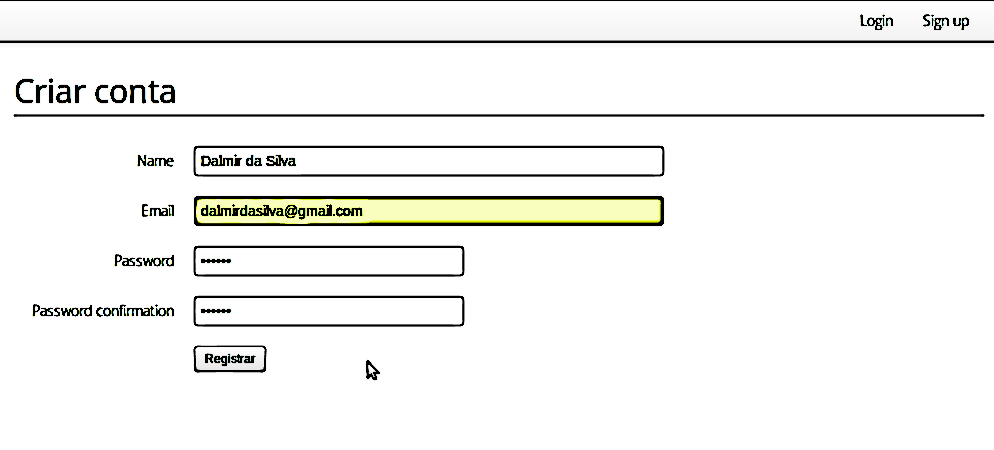
\includegraphics[width=.9\textwidth]{create_user.png}
      \caption{Tela de cadastro de novo usuário.}
    \end{figure}
    
    \subsection{Tela de autenticação do usuário.}
    
    \paragraph{}

    Nessa tela, um usuário já cadastrado pode se autenticar no sistema.
        
    \begin{figure}[h!]
      \centering
      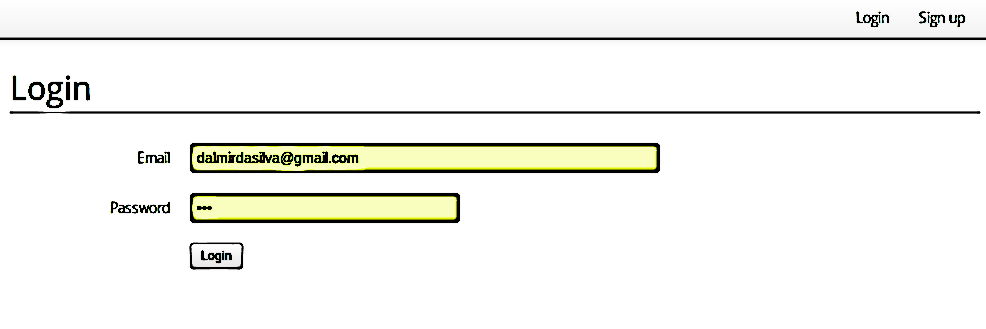
\includegraphics[width=.9\textwidth]{authenticate_user.png}
      \caption{Tela de autenticação do usuário.}
    \end{figure}
        
  \clearpage
    
    \subsection{Tela de criação de um novo formulário.}
    
    \paragraph{}

    Na tela seguinte, um usuário autenticado insere um novo formulário no
    sistema. Note que nessa tela apenas os dados básicos do formulário 
    podem ser inseridos, as perguntas e opções são inseridas na tela de 
    edição de formulário.
        
    \begin{figure}[h!]
      \centering
      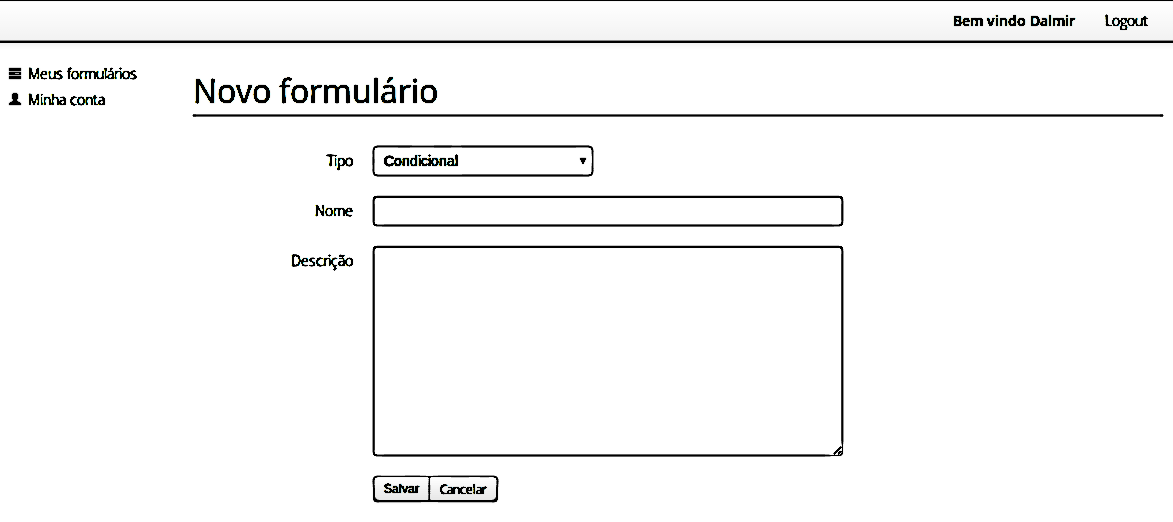
\includegraphics[width=.9\textwidth]{new_form.png}
      \caption{Tela de criação de um novo formulário.}
    \end{figure}
        
  \clearpage
    
    \subsection{Tela de edição do formulário.}
    
    \paragraph{}
    Essa tela é a principal tela do sistema. Nela, pode-se cadastrar e
    editar perguntas de um formulário. Perguntas podem ser de diferentes
    tipos. Na coluna à direita, são listados os diferentes tipos de 
    perguntas. Para adicionar uma nova pergunta ao formulário, basta clicar
    no botão correspondente à pergunta desejada.
    
    \paragraph{}
    Após adicionar uma pergunta, pode-se adicionar opções de resposta
    para ela - caso tal pergunta não seja de texto livre. Opções podem 
    ser removidas ou editadas. Para cada opção, pode-se adicionar uma 
    regra. Uma regra direciona o fluxo do questionário. Portanto, na regra
    pode-se definir o  número da próxima pergunta.
        
    \begin{figure}[h!]
      \centering
      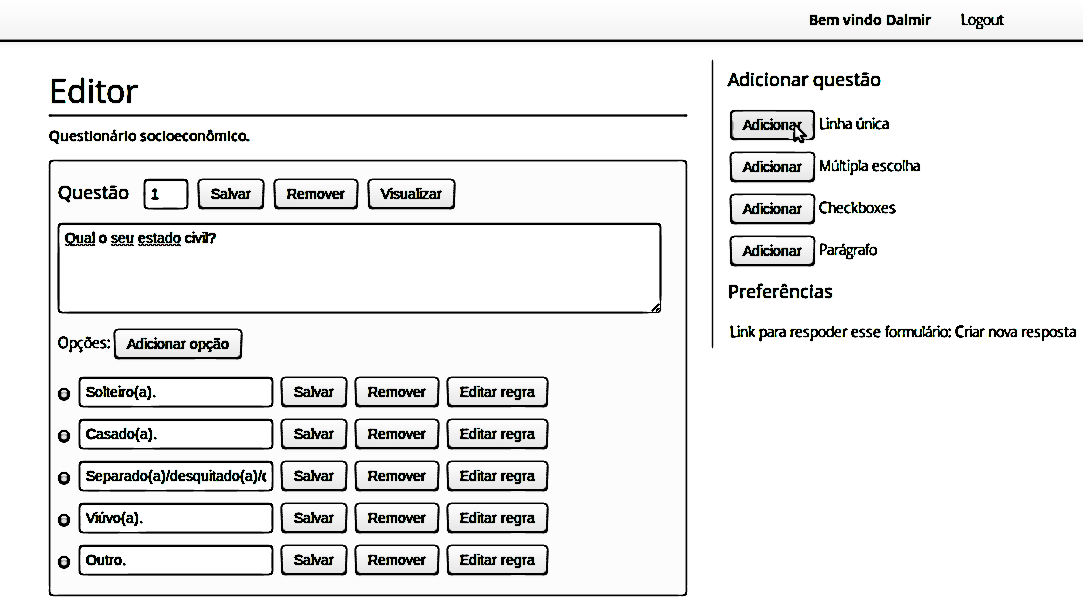
\includegraphics[width=.9\textwidth]{editor.png}
      \caption{Tela de edição do formulário.}
    \end{figure}
        
  \clearpage
    
    \subsection{Tela de resposta à um formulário.}
    
    \paragraph{}
    Essa é a tela de resposta para um determinado formulário. Como formulários
    podem ser contínuos ou condicionais, essa tela pode exibir as questões 
    do formulário de duas maneiras distintas. A figura a seguir, apresenta
    a tela de resposta de um questionário do tipo condicional. Nela, 
    a primeira pergunta do formulário é exibida e, dependendo da resposta, 
    outras novas peguntas são exibidas sessessivamente, se opondo ao modo de exibição de um 
    formulário contínuo, onde todas as perguntas são exibidas de uma só vez.
        
    \begin{figure}[h!]
      \centering
      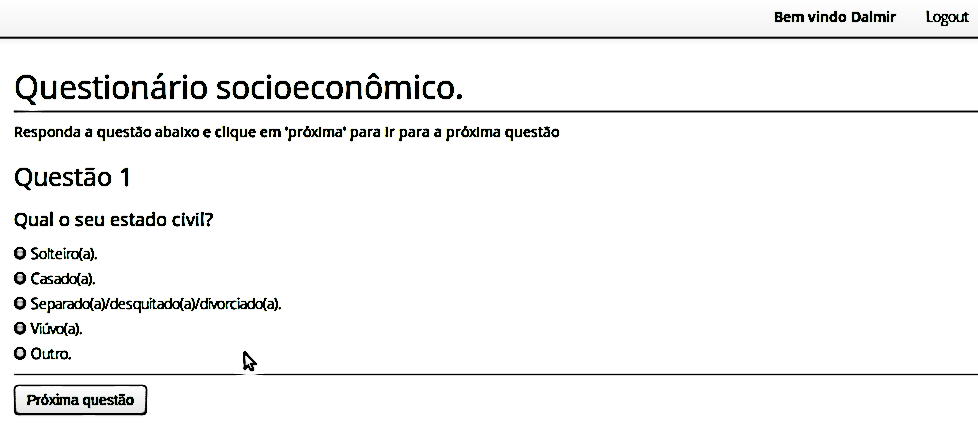
\includegraphics[width=.9\textwidth]{reply_a_form.png}
      \caption{Tela de resposta à um formulário.}
    \end{figure}
    
    \subsection{Tela de visualização de relatório.}
    
    \paragraph{}
    A próxima tela, é responsável pela visualização do relatório de respostas
    de um determinado formulário.
        
    \begin{figure}[h!]
      \centering
      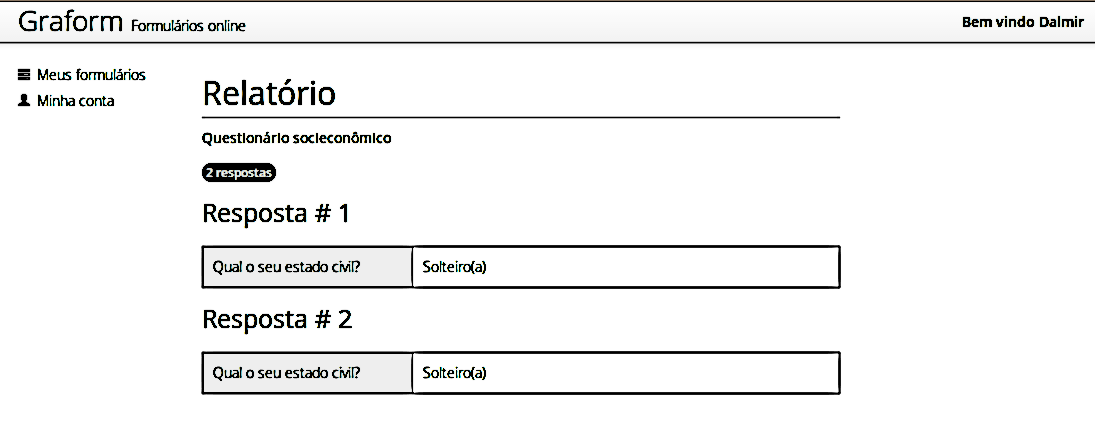
\includegraphics[width=.9\textwidth]{view_report.png}
      \caption{Tela de visualização de relatório.}
    \end{figure}
        
  \clearpage
      
  \section{Testes do sistema}
  
    \subsection{Desenvolvimento orientado a testes ({\em Test Driven Development})}
    
    \paragraph{}

    Como padrão de testes do projeto, utilizou-se {\em Test Driven 
    Development} (TDD). TDD é um padrão de testes no qual os testes são
    criados antes da implementação. Sendo assim, os testes orientam o
    codificação (como o nome já diz). Primeiro cria-se um teste, depois 
    criamos uma implementação para fazer o teste passar \cite{urubatan}.
     
    \subsubsection{{\em Rspec}}
  
    \paragraph{}

    TDD é uma proposta de desenvolvimento de software, e não uma 
    ferramenta de teste. Para isso, utilizou-se o {\em Rspec}. {\em Rspec}
    é um conjunto de ferramentas para testar a aplicação, direcionada para o
    {\em framework} Ruby on Rails.
    
    \paragraph{}
    
    Como o Ruby on Rails é um {\em framework} MVC, o {\em Rspec} provê um
    feramental para testar cada camada da aplicação.
        
  \clearpage
    
    \subsection{Testes dos modelos}
    
    \subsubsection{Usuário}
      
    \paragraph{}
    No próximo trecho de código, podemos ver um exemplo te teste do modelo
    Usuário:
    
    {\scriptsize
      \lstset{language=Ruby}
      \begin{lstlisting}

  require 'spec_helper'

  describe User do

    before :each do
      @user = User.new
    end

    describe "associations" do
    
      it 'should be associated with forms' do
        @user.should respond_to(:forms)
      end
    end

    describe "attributes" do

      it "should have name" do
        @user.should respond_to(:name)
      end

      it "should have email" do
        @user.should respond_to(:email)
      end

      it "should have password" do
        @user.should respond_to(:password)
      end
    end
  end
      \end{lstlisting}
    }
    
    \paragraph{}
    
    Neste teste, procura-se testar as relações do modelo com as outras 
    classes do sistemas, além de seus atributos.
    
    \paragraph{}
    Quando rodamos esse teste usando o {\em rspec}, temos a seguinte saída
    como resultado, mostrando que todos os testes passaram:
    
    {\scriptsize
      \lstset{language=sh}
      \begin{lstlisting}

  rspec --format nested spec spec/user

  User
    associations
      should be associated with forms
    attributes
      should have name
      should have email
      should have password

  Finished in 0.03836 seconds
  4 examples, 0 failures

      \end{lstlisting}
    }
        
  \clearpage
    
    \subsubsection{Fomulário}
      
    \paragraph{}
    A seguir, vemos os testes do modelo Formulário. Esse modelo possui, além
    dos testes de relacionamento e atributos, um método especial: $max\_question\_number$. 
    \\Esse método é responsável por retornar a questão desse formulário com maior número. 
    
    {\scriptsize
      \lstset{language=Ruby}
      \begin{lstlisting}
      
  require 'spec_helper'

  describe Form do

    before :each do
      @form = Form.new
    end

    describe "associations" do
    
      it 'should be associated with questions' do
        @form.should respond_to(:questions)
      end
    
      it 'should be associated with replies' do
        @form.should respond_to(:replies)
      end
    end

    describe "attributes" do

      it "should have a name" do
        @form.should respond_to(:name)
      end

      it "should have a description" do
        @form.should respond_to(:description)
      end
    end
    
    describe "#max_question_number" do
    
      it "should return the higest number of the existing questions" do
        @form.id = 1
        q0 = Question.new(form_id: @form.id, number: 0)
        q1 = Question.new(form_id: @form.id, number: 5)
        q2 = Question.new(form_id: @form.id, number: 4)
        @form.max_question_number.should == q1
      end
    end
  end
      \end{lstlisting}
    }
    
  \clearpage
    
    \paragraph{}
    
    O resultado do teste:
    
    {\scriptsize
      \lstset{language=Bash}
      \begin{lstlisting}

  rspec --format nested spec spec/form
      
  Form
    associations
      should be associated with questions
      should be associated with replies
    attributes
      should have a name
      should have a description
    #max_question_number
      should return the higest number of the existing questions


  Finished in 1.03234 seconds
  5 examples, 0 failures
      \end{lstlisting}
    }
    
    \paragraph{}
    
    A seguir, vemos o resultados de todos os testes rodados de uma
    só vez:
    
    {\scriptsize
      \lstset{language=Bash}
      \begin{lstlisting}

  rspec --format nested 
  
  User
    associations
      should be associated with forms
    attributes
      should have name
      should have email
      should have password

  Form
    associations
      should be associated with questions
      should be associated with replies
    attributes
      should have a name
      should have a description
    #max_question_number
      should return the higest number of the existing questions

  FormType
    associations
      should be associated with forms
    attributes
      should have a name
      should have a code

  Reply
    associations
      should be associated with answers
      should be associated with form
    
  Question
    associations
      should be associated with rules
      should be associated with options
    attributes
      should have a text
      should have a form
      should have a type
    #next_question
      when the form is continuous
        should get the next based on number
      when the form is conditions
        should get the next based on answer and the rule
      \end{lstlisting}
    }
    
    
  \clearpage
      
  \section{Conclusão}

    \paragraph{}
    Encontramos, ao longo do desenvolvimento desse projeto, inúmeras 
    circunstâncias onde as técnicas de desenvolvimento de software, 
    estudadas durante o curso, foram fundamentais para prover a melhor 
    solução para cada problema encontrado.
    
    \paragraph{}
    Técnicas, como TDD, propiciaram um desenvolvimento ágil e com boa taxa 
    de cobertura de código. Assim como o uso do padrão MVC ajudou no objetivo de atingir baixo acoplamento
    e alta coesão das classes do sistema.
    
    \paragraph{}
    A utilização de uma aplicação web, possível de ser acessada por
    qualquer computador, sem a necessidade de instalação de um software 
    {\em desktop}, aumentou a produtividade da empresa como um todo. Também,
    houve uma redução de incidências de erros humanos, devido ao fato de não ser mais necessáro o
    uso de instrução SQL diretamente na base de dados para a criação e gerenciamento dos formulários.

  \newpage
  \bibliography{project}{}
  \bibliographystyle{plain}
  
\end{document}

